\chapter{ПРАКТИЧЕСКАЯ РАБОТА № 6 <<ДИАГРАММЫ КОНЕЧНОГО АВТОМАТА И ДИАГРАММЫ СОСТОЯНИЙ>>}

\section{Цель работы}

Целью данной практической работы является ознакомление с семантикой диаграммам схем конечных автоматов и диаграмм состояний в контексте UML.

\section{Теоретические сведения}

Диаграмма конечных автоматов предназначена, прежде всего, для описания процесса изменения состояния конкретного объекта, а если быть точным для описания различных состояний, в которых может находиться объект, и переходы между этими состояниями. Диаграмма конечных автоматов позволяет описать поведение конкретного объекта модели (реакции объекта на возможные внешние и внутренние изменения), посредством описания всех возможных последовательностей состояний и переходов в рамках конкретной модели разрабатываемой системы. Основным достоинством диаграммы состояния является то, что она позволяет описать динамическое поведение сущностей (объектов и т.д.) при воздействии на эти сущности внешнего и внутреннего воздействия, как было выяснено выше, на всем этапе жизненного цикла данной сущности.

Наиболее часто на практике данные диаграммы используются в объектно-ориентированной парадигме для описания динамического поведения конкретного экземпляра класса (объект), но при этом данные диаграммы могут совместно использоваться с различными диаграмми UML в комбинациях, что позволяет, например, в случае комбинации с диаграммами вариантов использования описать функциональные ограничения в поведении актёра.

Диаграммы конечного автомата UML изображают различные состояния, в которых может находиться объект, и переходы между этими состояниями. Фактически, в других языках моделирования этот тип диаграммы обычно называют диаграммой перехода состояний или даже просто диаграммой состояний. В нотации UML используются диаграммы состояний Харела, которые позволили обойти ограничение классических диаграмм состояний, которое связано со снижением удобочитаемости классических диаграмм при увеличении количества узлов и переходов между узлами для всех систем. При этом диаграмма состояний Харела эквивалентна классической диаграмме состояний. 

Диаграммы состояний требуют, чтобы описываемая система состояла из конечного числа состояний и позволяют, используя граф специального вида (ориентированный граф), в которых вершины (узлы) обозначают состояния, а дуги обозначают переходы состояний, графически описать представление конечных автоматов. 

В нотациях UML состояния представлены в виде скругленных прямоугольников, которые помечены именами состояний. Переходы, обозначены стрелками, помечены запускающими событиями, за которыми необязательно следует список выполненных действий. Начальный переход происходит из сплошного круга и определяет начальное состояние.

\subsection{Состояния и композитные состояния}

Состояние моделирует ситуацию, при которой выполняется некоторое инвариантное условие. В большинстве случаев это условие не определено явно.

Выделяют следующие типы состояний:

\begin{enumerate}
	\item{Простое состояние (не имеет внутренних вершин или переходов)}
	\item{Составное состояние (содержит хотя бы один регион)}
	\item{Субмашинное состояние}
\end{enumerate}

\subsection{Внутреннее поведение}

Внутреннее поведение содержит список внутренних действий или действий состояния (do), которые выполняются, пока элемент находится в этом состоянии. Каждое из этих внутренних действий записывается в формате <метка-действия '/' выражение-действия>. Метка действия часто представляет собой то условие при которых данное выражение-действие будет выполнено.

Несколько меток зарезервированы для специальных целей и не могут использоваться в качестве имен событий. Ниже перечислены зарезервированные ярлыки действий:

\begin{itemize}
	\item{entry}
	\item{do}
	\item{exit}
\end{itemize}

\subsection{Начальное и конечное состояние}

Начальное псевдосостояние представляет собой отправную точку, в которой находится объект в начальный момент времени и служит для отображения той графической области, которая будет являться областью изменения состояния. При этом, в данной области не может быть более одной начальной вершины.

Конечное состояние --- это особый вид состояния, которое не содержит никаких внутренних действий. 

\subsection{Переход и виды переходов}

Переход представляет собой направленные отношения между исходной и целевой вершинами (состояния). В зависимости от отношения к вершине в общем случае выделяют 3 основных вида переходов:

\begin{enumerate}
	\item{ external --- переход выходит из своей исходной вершины (выполняет действие выхода из исходного состояния)}
	\item{local ---- переход не выходит из содержащего его состояния (действие выхода из содержащего состояния не будет выполнено), при этом локальный переход может существовать только в составном состоянии}
	\item{ internal переход является частным случаем локального перехода с одинаковыми исходным и целевым состояниями}
\end{enumerate}

\section{Задание на практическую работу}

 Используя средства UML, необходимо разработать диаграмму состояний для класса «Заказ» из предыдущей практической работы.

\section{Выполнение практической работы}

\begin{figure}[h!]
        \centering
        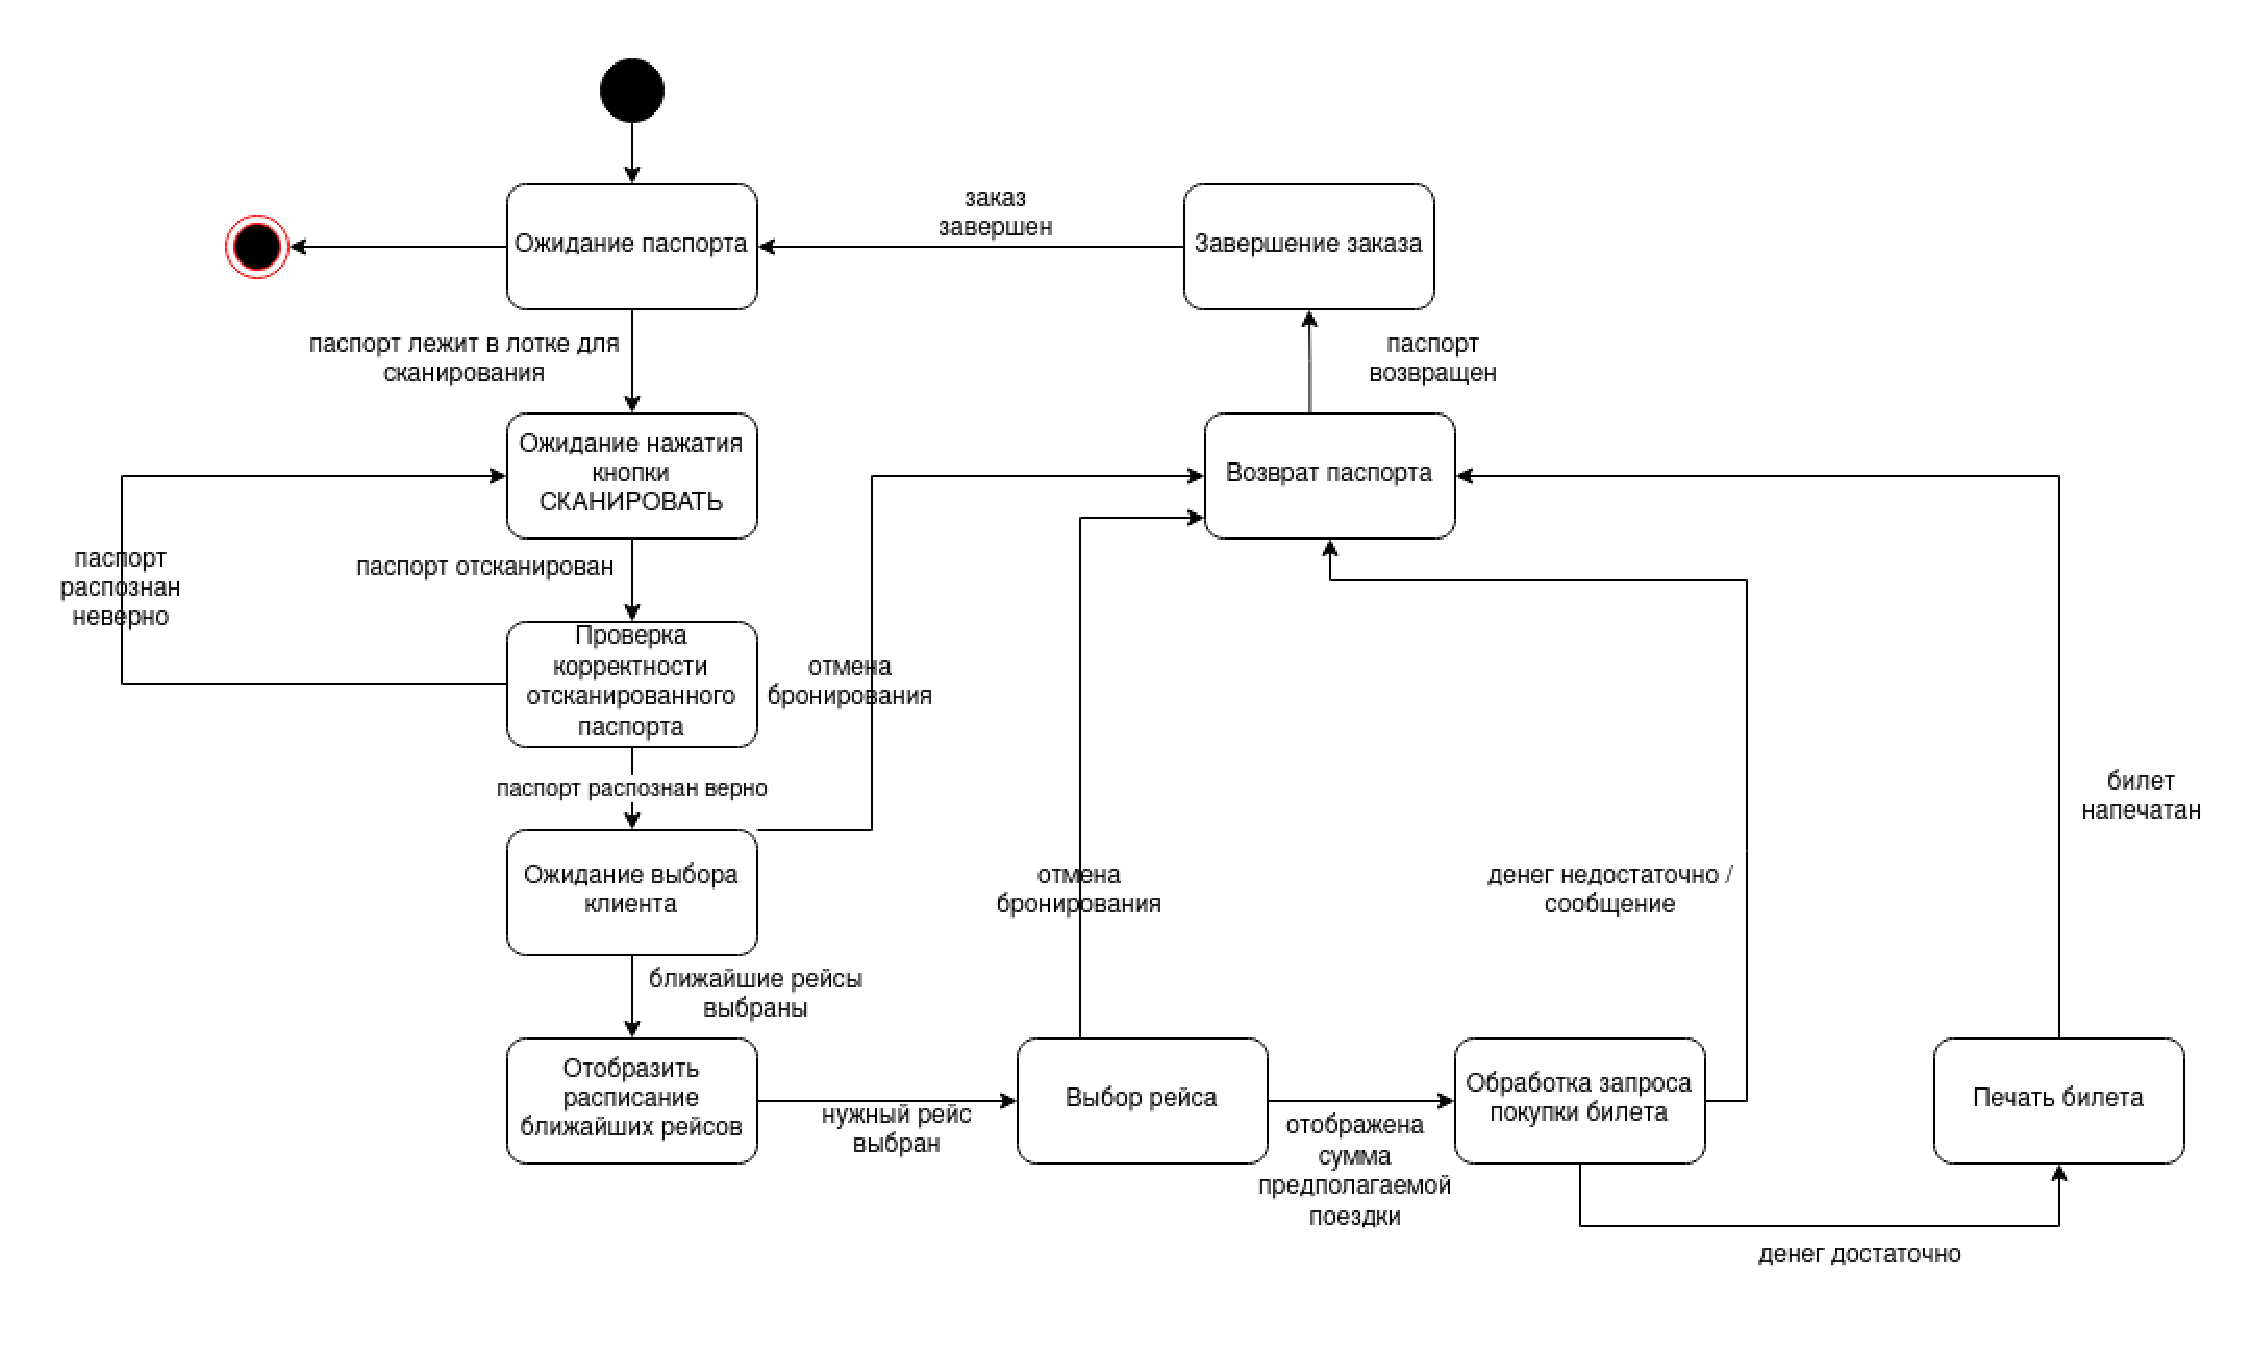
\includegraphics[width=0.7\textwidth]{images/6/state.eps}
        \caption{Диаграмма состояний объекта}
        \label{state}
\end{figure}

\newpage

\section{Вывод}

Ознакомились с семантикой диаграммам схем конечных автоматов и диаграмм состояний в контексте UML.
